\section{\"{A}nderungen gegen\"{u}ber dem Entwurf}

\subsection{Paket\"{a}nderungen}
\begin{itemize}
  \item Das Interface ASTVisitor wurde vom interpreter- in das ast-Paket verschoben, da das Interface logisch unabh\"{a}ngig vom Interpreter ist.
  \item Ebenso wurden der TypeChecker und die hiervon verwendete IllegalTypeException in das parser-Paket verschoben, da beide Klassen haupts\"{a}chlich beim Parse-Vorgang verwendet werden.
  \item Der SMTLib-Translator wurde vom interpreter- in das verifier-Paket verschoben, da dieser wesentlicher Bestandteil der Verifikation ist und unabh\"{a}ngig vom Interpreter ist.
  \item Die Klasse MessageSystem befindet sich nicht mehr im interpreter-Paket, sondern im misc-Paket, da sie als Modell dient.
\end{itemize}

\subsection{Paket ast}
\begin{itemize}
  \item Assignment hat ein zus\"{a}tzliches Attribut \code{depth} zur Repres\"{a}ntation der Scopetiefe der Variablendeklaration.
  \item ArrayType hat eine zus\"{a}tzliche Assoziation zu Type mit der Rolle \code{basetype}. Hiermit werden unterschiedliche Arraytypen, wie z.B. \code{bool[]}, \code{int[]} und \code{int[][]}, unterschieden.
  \item Die Klasse Length wurde gel\"{o}scht, da diese nun in den Visitorklassen als spezieller Funktionsaufruf behandelt wird.
  \item FunctionCall hat eine zus\"{a}tzliche Assoziation zu Identifier, welche vom TypeChecker zur Referenzaufl\"{o}sung verwendet wird. Hierdurch ist auch die Methode \code{setFunction} zur Klasse hinzugef\"{u}gt worden.
  \item Loops k\"{o}nnen nun neben Invarianten auch Ensures beinhalten, die als Nachbedingungen nach Schleifenende gepr\"{u}ft werden und f\"{u}r eine Verifikation bewiesen werden m\"{u}ssen.
  \item Functions haben die M\"{o}glichkeit Assumptions und Ensures zu besitzen. Assumptions stellen hierbei Vorbedingungen, Ensures Nachbedingungen dar. Beide Zusicherungen sind f\"{u}r einen Korrektheitsbeweis n\"{o}tig. Verwendet man Assumptions in der \code{main}-Funktion, so kann man den Parameterbereich f\"{u}r den Beweiser einschr\"{a}nken.
  \item Die Klasse Range wurde neu eingef\"{u}hrt, welche zwei Assoziationen \code{lower} und \code{upper} zu Expression besitzt. Die Klasse dient zur Einschr\"{a}nkung des Bereichs in quantifizierten Ausdr\"{u}cken. Infolgedessen haben QuantifiedExpressions eine Assoziation zu Range.
  \item BooleanLiteral und IntegerLiteral speichern ihre Werte im neuen \code{value}-Attribut vom Typ Value.
  \item Das Interface ASTVisitor kann nun auch StatementBlocks mit der \code{visit}-Methode besuchen.
  \item Die Klasse QuantifiedExpression erbt nun von LogicalExpression, da jede QuantifiedExpression ein Boolean zur\"{u}ck gibt.
  \item Die Indizes aller Array-Klassen wurden vom Typ ArithmeticExpression zu Expression ge\"{a}ndert, die Bedingung von Loops und Conditionals ebenfalls von LogicalExpression zu Expression. Dies erm\"{o}glicht es nun auch Variablen bzw. Arraykomponenten und gegebenenfalls auch Funktionsaufrufe in diesen F\"{a}llen zuzulassen. Die Typsicherheit wird durch den TypeChecker sichergestellt.
  \item Die Klassen LogicalOperator und ArithmeticOperator wurden zu Interfaces, die von den bisherigen Kindklassen implementiert werden. Zus\"{a}tzlich erben die Kindklassen von einem der beiden neuen Klassen UnaryOperator bzw. BinaryOperator.
  \item Die Methode \code{getNextStatement} in StatementBlock wird ersetzt durch eine neue Methode \code{getIterator}, die einen Iterator f\"{u}r die Statements in diesem StatementBlock zur\"{u}ckgibt. Dies entkoppelt die Klasse des Syntaxbaums von einer konkreten Abarbeitung.
  \item Die Klasse UnaryPlus wurde als unn\"{o}tig identifiziert und somit entfernt.
\end{itemize}

\subsection{Paket parser}
\begin{itemize}
  \item Neue Exception FunctionCallNotAllowedException, die geworfen wird, wenn Funktionsaufrufe an einer Stelle stehen, an der sie nicht erlaubt sind. Infolgedessen hat der TypeChecker ein neues Attribut \code{functionCallAllowed} mit Getter- und Setter-Methode.
  \item Die Klasse TypeChecker bekommt ein neues Attribut \code{currentScope} vom Typ Scope und eine dazugeh\"{o}rige Setter-Methode, die bei der Auswertung von GlobalBreakpoints benutzt wird.
  \item Die Klasse IllegalTypeException ist zur besseren Anzeige mit einer Position assoziiert.
\end{itemize}

\subsection{Paket interpreter}
\begin{itemize}
  \item Die neuen Klassen BooleanValue, IntegerValue und ArrayValue erben von der Klasse Value und repr\"{a}sentieren einen Boolean-Wert durch ein Attribut vom Typ \code{boolean}, eine Ganzzahl durch ein Attribut vom Typ \code{BigInteger} bzw. ein Array durch ein Array vom Typ \code{Value[]}.
  \item Die Klasse GlobalBreakpoint hat nun eine Assoziation zur Klasse Expression statt zu LogicalExpression. Dies erm\"{o}glicht es nun auch Variablen bzw. Arraykomponenten und gegebenenfalls auch Funktionsaufrufe in globalen Breakpoints zuzulassen. Die Typsicherheit wird durch den TypeChecker sichergestellt.
  \item Die Klasse StatementBreakpoint ist nicht mehr einem Statement, sondern eine Zeile zugeordnet, da hierdurch die Breakpointbehandlung vereinfacht wird.
  \item Die Klasse Scope:
  \begin{itemize}
    \item hat ein neues Attribut \code{returnValues} vom Typ IdentityHashMap zur Speicherung von Zwischenergebnissen von Funktionsaufrufen und eine zugeh\"{o}rige Getter-Methode.
    \item hat ein neues Attribut \code{currentFunction} vom Typ Function zur Identifizierung der zum Scope zugeh\"{o}rigen Funktion, falls vorhanden.
    \item hat ein neues Attribut \code{statements} vom Typ Iterator<Statements> zum Iterieren \"{u}ber Statements unabh\"{a}gig von anderen Scopes, was insbesondere bei Rekursionen wichtig ist.
    \item hat ein neues Attribut \code{currentStatement} vom Typ Statement zum Speichern des momentanen Statements im Fall eines Funktionsaufrufs und eine zugeh\"{o}rige Getter-Methode.
    \item hat aufgrund der neuen Attribute einen ge\"{a}nderten Konstruktor.
    \item hat eine neue Methode \code{isFunctionScope} zur Feststellung, ob ein Funktionsscope am Ende einer Funktion abgebaut wird.
    \item hat eine neue Methode \code{getCurrentFunction}, die die Funktion zur\"{u}ckgibt, in der der Scope bzw. ein \"{u}bergeordneter Scope ist.
    \item hat eine neue Methode \code{createVar} zum Erzeugen von Variablen und eine neue Methode \code{createArray} zum Erzeugen von Arrays. Infolgedessen gibt es getrennte Methoden \code{setVar} und \code{setArray} zur \"{A}nderung der Werte der Variablen bzw. Arrays.
    \item hat eine neue Methode \code{createFunctionResult} zur Berechnung neuer Ergebnisse f\"{u}r \code{returnValues}.
    \item hat eine neue Methode \code{clearFunctionResult} zum L\"{o}schen der Zwischenergebnisse in \code{returnValues}.
  \end{itemize}
  \item Infolge der \"{A}nderungen der Klasse Scope wurde in der Klasse State die Parameter der Methoden \code{createScope}, \code{setVar} und \code{createVar} angepasst und die Methoden \code{createArray}, \code{setArray}, \code{getCurrentFunction}, \code{isFunctionScope} und \code{getReturnValues} hinzugef\"{u}gt. Au\ss erdem gibt es eine neue Methode \code{adjustStatement}, die das n\"{a}chste Statement bestimmt und setzt.
  \item Die Klasse ProgramExecution:
  \begin{itemize}
    \item die Methode \code{setBreakpoint} wurde entfernt. Zur besseren Behandlung der beiden Breakpoint-Typen existieren nun Assoziationen zu GlobalBreakpoint und StatementBreakpoint. F\"{u}r die \"{U}berpr\"{u}fung von globalen Breakpoints besitzt die Klasse nun ein Attribut vom Typ TypeChecker. Aufgrund der \"{A}nderungen wurde der Konstruktor der Klasse angepasst.
    \item die Methode \code{checkBreakpoint} liefert nun im Fall eines getroffenen Breakpoints den jeweiligen Breakpoint zur Anzeige zur\"{u}ck.
    \item hat neue Methoden \code{initParams} und \code{initArray} zur Initialisierung von Parametern der \code{main}-Funktion.
  \end{itemize}
  \item Die Klasse Interpreter hat eine innere Klasse StopStatementExecution, die zum Abbrechen des aktuellen Statements bei Funktionsaufrufen benutzt wird.
  \item Die Klasse Interpreter hat neue Methoden \code{adjustStatement} zur Anpassung des momentanen Statements und \code{checkAssumptions} zur Spezialbehandlung der Assumptions der \code{main}-Methode.
  \item Die Klasse AssertionFailureException ist zur besseren Anzeige mit einer Position assoziiert.
\end{itemize}

\subsection{Paket verifier}
Die Schnittstelle und Arbeitsweise des Beweiserpakets wurde w\"{a}hrend der Implementierungsphase ge\"{a}ndert, um eine h\"{o}here Flexibilit\"{a}t und Erweiterbarkeit erreichen.
\begin{itemize}
  \item Neue Klasse Verifier als Basisklasse und einheitliche Schnittstelle f\"{u}r einen Beweiser. Die Klasse Z3 erbt von dieser Klasse.
  \item Neue Klasse VerifierInterface als Fassade des verifier-Pakets nach au\ss en.
  \item Neue Klassen VarDef und Variable, die von S\_Expression erben und zur Ersetzung im wp-Kalk\"{u}l dienen.
  \item Die Klasse S\_Expression hat eine neue Methode \code{deepCopy}, die referenzungleiche Kopien einer S\_Expression und ihrer Subexpressions erzeugt.
  \item Die Klasse SMTLibTranslator hat neue Methoden \code{prepareFinalProgram} und \code{createBlock} zum Abschluss des \"{U}bersetzungsvorgangs.
\end{itemize}
Aufgrund der gr\"{o}\ss eren \"{A}nderungen folgt ein vereinfachtes aktuelles Klassendiagramm des Paketes:\\
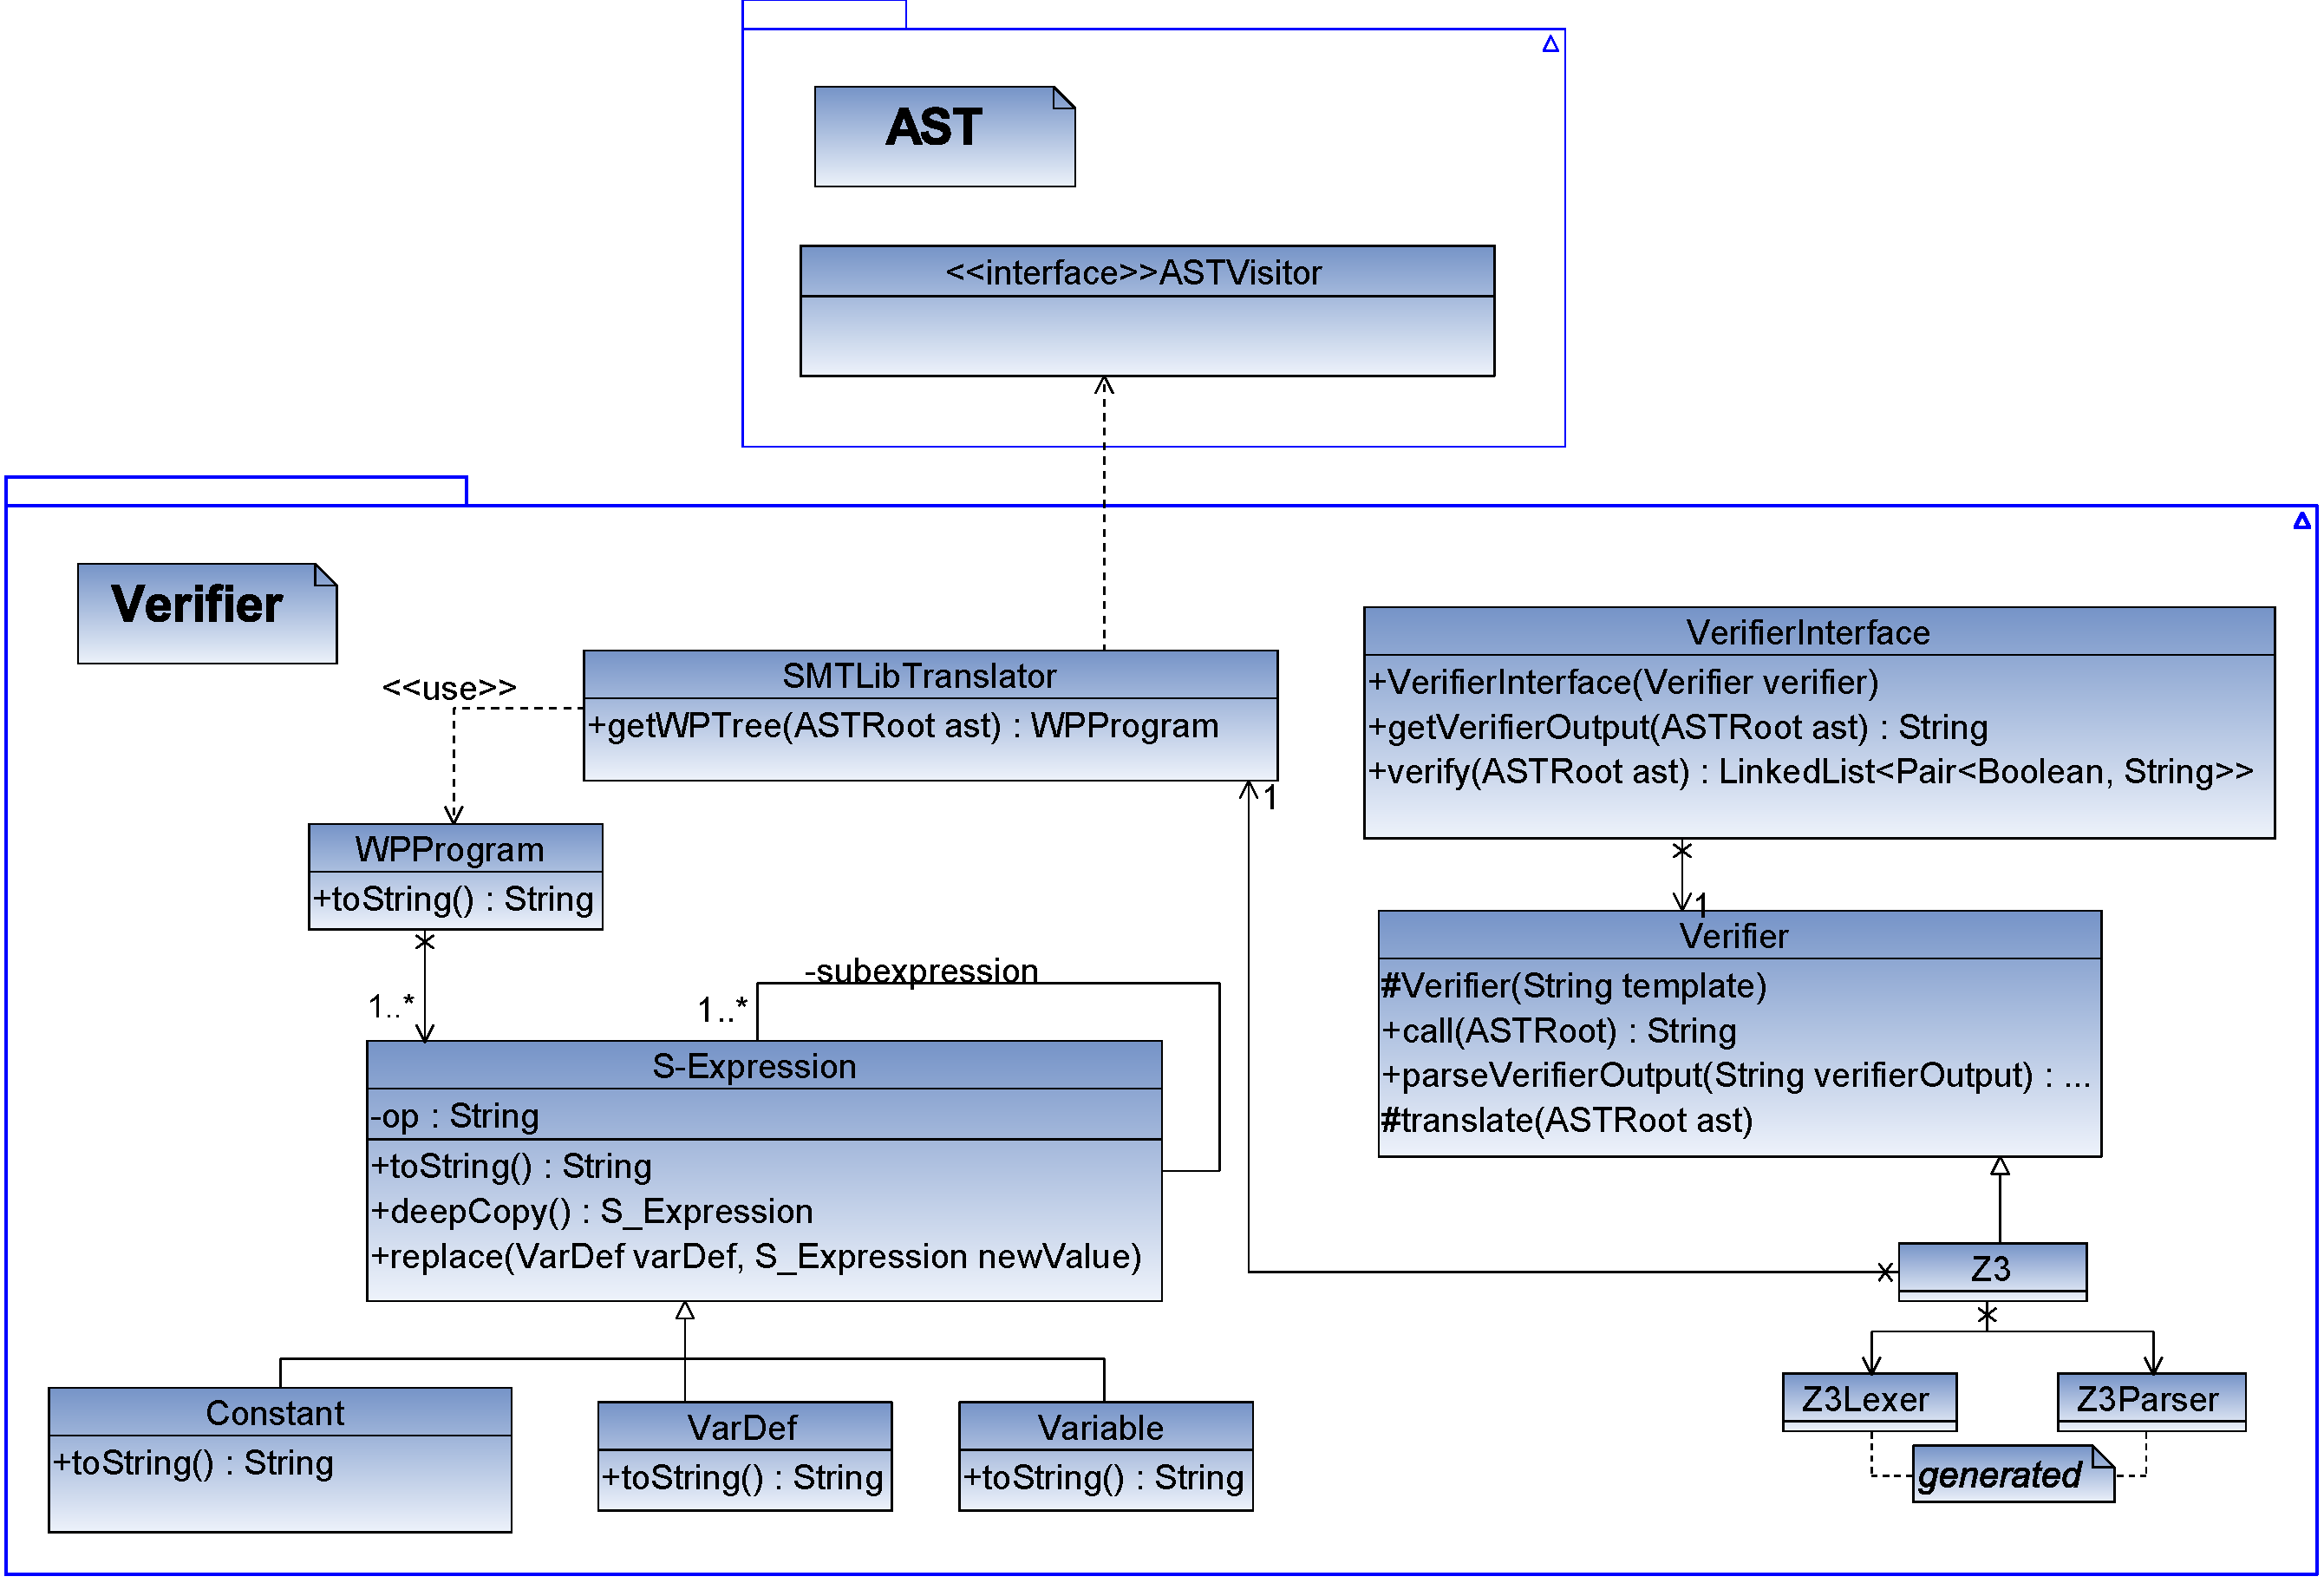
\includegraphics[width=0.8\paperwidth]{images/Verifier.pdf}

\subsection{Pakete gui und misc}
Die Pakete der GUI-Komponente wurden w"ahrend der Implementierungsphase nochmals "uberarbeitet. Der urspr"ungliche Entwurf war nicht auf das verwendete Toolkit SWT ausgelegt, deswegen wurden die Attribute und Methoden der meisten Klassen des gui-Pakets angepasst. Auch an der gesamten Klassenstruktur mussten einige Ver"anderungen vorgenommen werden. Die Bestandteile des MVC-Patterns wurden zum Teil nicht klar getrennt und der Entwurf erschien dadurch inkonsistent. Die wichigsten "Anderungen sind im Folgenden aufgelistet. 
\begin{itemize}
\item Die Klasse ExecutionController wurde zu ExecutionHandler umbenannt, da der alte Name leicht mit einem Controller des MVC-Patterns verwechselt werden konnte und die Klasse in Wirklichkeit nicht die Rolle des Controllers spielt. Auf Grund ihrer Teilfunktion als Modell wurde sie in das misc-Paket verschoben.
\item Die Funktionen Parsen, Interpretieren und Validieren werden nun alle vom ExecutionHandler aufgerufen und nicht, wie im Entwurf, zum Teil vom MainController. Diese "Anderung war wichtig, da wir nun die Funktionen einheitlich behandeln k"onnen. So ist der MainController nur noch f"ur die Inizialiserung des MainFrames und aller anderen Controller zust"andig. 
\item Assoziationen zwischen diversen Controllern und der ProgramExecution des interpreter-Pakets wurden aufgel"ost und durch eine ExecutionHandler-ProgramExecution-Assoziation ersetzt. So konnte die Verbindung zwischen der GUI und dem Rest des Systems gelockert werden.
\item VariableViewController und BreakpointViewController wurden zusammen gefasst zu TableViewController, da sie das selbe Modell benutzen. 
\item Die urspr"ungliche Editor-Klasse war View, Controller und Modell zugleich. Dies wurde verbessert und dadurch sind die Klassen Editor (als Modell), EditorController und EditorView entstanden.
\item Der MiscController hat an Bedeutung verloren und entsprach nicht mehr dem aktuellen Entwurf, deshalb wurde die Klasse entfernt. Stattdessen haben die Frames, die gesteuert werden m"ussen, ihren eigenen Controller bekommen. Deswegen wurde das gui-Paket durch die Klassen HelpController, ParameterController und SettingsController erg"anzt.
\item Es wurden die Klassen ParameterFrame und ParameterController hinzugef"ugt, da nicht an die "Ubergabe der Parameter an die Main-Funktion gedacht wurde. Dies ist nun durch das "Offnen eines ParameterFrames m"oglich.
\end{itemize}
Aufgrund der gr\"{o}\ss eren \"{A}nderungen folgt ein aktuelles Klassendiagramm des Paketes:\\
\begin{landscape}
\includegraphics[width=0.85\paperheight]{images/coregui.pdf}
\end{landscape}
\subsection{While-Sprache}
\begin{itemize}
\item Zur Vereinfachung der Behandlung von Funktionsaufrufen im SMTLibTranslator wird ein Return-Statement nur noch am Ende von Funktionen (die main-Funktion ausgeschlossen) erlaubt.
An diesen Stellen muss dieses Statement sogar stehen, sonst ist das Programm nicht syntaktisch korrekt. Dies wird schon im Parser erkannt.
\item Funktionsaufrufe in Assumptions, Axioms, Ensures, Invariants und QuantifiedExpressions werden verboten, nur noch die eingebaute \"length\"-Funktion ist erlaubt. 
Neben einer Vereinfachung des Beweisers dient dies auch der Benutzerfreundlichkeit. 
Durch die Funktionen müsste nämlich intern im Single-Step-Modus durchgegangen werden, um jederzeit eine Unterprechung des Programmablaufs zu erlauben.
Da die QuantifiedExpression aber eventuell über einen sehr großen Bereich geprüft wird, ist dies für den Benutzer ein zu großer Aufwand. Die restlichen Statement-Arten
werden außerhalb eines Statements gemeinsam geprüft. Ein Funktionsaufruf im Singlestep wäre gegen die Logik dieser Statements.
\item Die Syntax der Arraydeklaration wurde geändert, da die Syntax im Entwurf unintuitiv war.
\end{itemize}